\documentclass{article}
\usepackage{import}
\subimport{../}{preamble}
\begin{document}

%\fullcite{bharadwaj2009}

\section{Plasmons in Tips}
\label{sec:tip_literature}

Significant efforts have been made to advance surface characterisation on the nm-scale by developing new optical tools and integrating optics into existing nanoscale topological measurements. Metallic tips were  investigated due to the widespread use of \glspl{spm}, such as \gls{afm}, and \gls{stm}. The similarity in size between metallic nanostructures and the small apex of tips initially suggested that visible plasmons would be expected, enabling resonant near-field enhancement.
% Application of tips to TERS and SNOM - keep this short, the thesis is not about Raman but this is a motivation
Prior to any spectral characterisation studies to understand the near-field response, tips were applied in combined SPM-optical microscopes to achieve sub-wavelength localisation and enhancement of optical signals. As the next logical step from \gls{sers} and \gls{snom}, the sharp apex of tips were exploited to develop the spin-off techniques of \gls{ters} \cite{stockle2000, anderson2000, hayazawa2000, pettinger2000} and \gls{asnom}%
\footnote{Also known as \gls{ssnom}.}
\cite{zenhausern1994, zenhausern1995, bachelot1995, knoll1997, knoll1998, keilmann1999}.
These are also known collectively as \gls{tenom}.%
\footnote{These are also sometimes known as field-enhancing near-field optical microscopy (FENOM) since apertured techniques do not necessarily exploit plasmonic enhancement as much.}

% TERS
The concept for \gls{tenom} was first proposed in 1985 \cite{wessel1985} but it was not until 2000 that the first reported uses of tips for enhancing Raman spectroscopy emerged \cite{stockle2000, anderson2000, hayazawa2000, pettinger2000}. All measurements were carried out in inverted microscopes with either an \gls{afm} \cite{stockle2000, anderson2000, hayazawa2000} or \gls{stm} \cite{pettinger2000} mounted on top. Two of the initial measurements suggest the overall Raman enhancement has a lower limit of $\sim$\num{e4} \cite{stockle2000, anderson2000}, hence a field enhancement \orderof{10}, whereas a third obtained an enhancement factor of 80 from a single tip apex excited using $\NA > 1$ evanescent waves, equivalent to the summed enhancement of many SERS hotspots on a Ag island film \cite{hayazawa2000}. Since then Raman enhancements in the region of \num{e7}--\num{e9} have been measured \cite{pettinger2012}.%
\footnote{A clear distinction is made between the field enhancement, $|E/E_0|$, and the Raman enhancement, $|E/E_0|^4$, when stating enhancement factors. In the literature the terms ``field enhancement" or ``enhancement factor" are generally used interchangeably between the magnitude of the near-field and the improvement in the Raman signal.}
Whilst SERS enhancement factors have also increased significantly in recent years, the \gls{tenom} approach to spectroscopy remains a popular technique since the tip can be scanned across a sample whereas SERS substrates are static. For this reason, techniques such as TERS are widely considered to become the successors of SERS. However, for this to be the case, nanotips require the capability to controllably and reproducibly enhance the near-field. Understanding the electromagnetic response of metallised tips has therefore become of significant importance in recent years.
Since the use of tips for plasmonics is a central part of this project it is important to understand the underlying concepts and mechanisms of \gls{tenom} as these inevitably influence any observed plasmonic behaviour.

\begin{figure}[bt]
%\centering
\flushleft
\fontsize{10pt}{1em}\selectfont
\begin{subfigure}[t]{0.47\textwidth}
	%\centering
	\subimport{./figures/}{tenom_basic}
\end{subfigure}
~
\begin{subfigure}[t]{0.49\textwidth}
	%\centering
	\subimport{./figures/}{tenom_surface}
\end{subfigure}
\caption[Concepts of TENOM]{\textbf{Concepts of TENOM.}
Tips can perturb evanescent surface waves and scatter them into the far-field ($1\rightarrow3$) \cite{neacsu2005, mehtani2006}.
Photons illuminating a tip-sample junction can induce a hot-spot, which scatters light into the far-field ($2\rightarrow3$).
SPPs coupled onto a planar metal surface (via a tip) can radiatively decay into $\mathit{NA}>1$ ($1\rightarrow4$) \cite{wang2011}.
{\color{red}Mechanism ($2\rightarrow4$) has not been attempted.}}
\label{fig:tenom_concept}
\end{figure}

\Gls{tenom} is ideally classified as a local excitation approach as opposed to a local scattering approach \cite{novotny2006}, though the two approaches are not independent. In the tip scattering approach the non-radiative near-field, comprising evanescent waves, is perturbed by the presence of the tip, leading to scattering into the far-field {\color{red}(same frequency as illumination but lower \wvm)}. In the tip excitation approach the tip is resonantly excited to induce a large local near-field enhancement and used as a sub-diffraction-limited light source, from which the localised scattering can be measured. This process can be much more efficient than the pure scattering approach but depends on the optical antennae properties of the tip. In both cases the resolution of scattering images is sub-diffraction limited and on the order of the tip radius. In most cases this means a sub-\SI{50}{nm} resolution.

\subsection{The Electromagnetic Response of Tips}

\begin{wrapfigure}{O}{0.45\textwidth}
\centering
\vspace{-15pt}
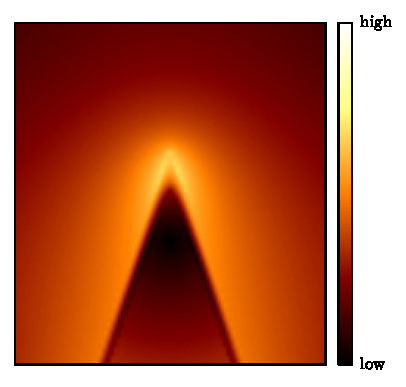
\includegraphics[width=\textwidth]{figures/lightning_rod_effect}
\vspace{-25pt}
\caption[Calculated magnitude of the electric field around a tip showing the lightning rod effect]{\textbf{Calculated magnitude of the electric field around a tip showing the lightning rod effect.} Compression of the field lines around the sharp corner of an equipotential surface leads to a localised, non-resonant field enhancement.%
\footnote{Poisson's/Laplace's equation is solved for a tip structured electrode with a surface charge distribution separated by some distance from a planar metal counter electrode of the opposite surface charge.}}
\label{fig:lightning_rod_effect}
\end{wrapfigure}

The electromagnetic response of tips can be broken down into individual components that constitute the enhancement mechanism. The two main optical components are a lightning rod effect and a resonant plasmon contribution for metallic tips \cite{esteban2006, zhang2009, schmid2013}. Each component is maximised when the incident field is along the tip axis \cite{zhang2014}. The main focus of recent tip work has been to study the plasmonic component, however progress in sharpening tips has led to increases in the lightning rod component. Both components are important to consider when attempting to understand optical measurements involving tips.

% The lightning rod effect in tips
Regardless of plasmonic behaviour, metallic tips intrinsically exhibit a lightning rod effect under the application of an applied field, instilling a non-resonant component of near-field enhancement. From the definition of the electric field $\vec{E}(\vec{r}) = -\nabla\pot(\vec{r})$ it is clear that the electric field strongly depends on geometry with field lines perpendicular to the equipotential conductor surface. The more curved a surface, the more compressed the field lines become around its surface due to accumulation of surface charge. This can be described by $E = \sigma/\epsfs$ where $\sigma = q/4\pi r^2$ is the surface charge density and $r$ is the radius of curvature. Since $E \propto 1/r^2$ the electric field is larger in regions of smaller  curvature. This effect is shown using a simple sharp tip model in \figurename~\ref{fig:lightning_rod_effect}. Consequently, even without a plasmonic component, sharp tips provide a promising platform for localised near-field enhancement.

% The plasmonic component
The expected plasmonic component arises from the curvature of the metal-dielectric interface at the tip apex. This allows for either the excitation of \glspl{spp} at the apex or for \glspl{spp} propagating towards the apex to localise due to adiabatic nanofocussing \cite{stockman2004, pile2006, berweger2010, lee2011, berweger2012, lindquist2013}. As highlighted when discussing ellipsoidal \glspl{mnp}, strong, antenna-like \glspl{lsp} are unlikely to exist at the apex of a sharp tip since lack of a second metal-dielectric interface prevents accumulation of the opposite surface charge to the apex. The tip can almost be described as a MI geometry as opposed to the \gls{imi} geometry that results in \glspl{lsp}. Thus there can be no strong restoring forces or \glspl{spr}. The extended size of the typical tip structure ($\sim$\SI{20}{\micro\metre}) also means that any potential low-order antenna modes would have to exist far in the IR. Simulations of shorter tip geometries show visible-NIR \glspl{lsp}, however these redshift and diminish with increasing tip length \cite{zhang2009, huber2014}. The standard, sharp metallic tip geometry therefore makes for a poor \textit{plasmonic} optical antenna unless \glspl{spp} can be excited. Despite this claim a large number of papers give convincing evidence for the presence of localised apex plasmons, such as depolarised scattering images \cite{mino2014}, however these typically have a degree of nanostructuring capable of sustaining more localised modes \cite{hayazawa2001, bailo2008, hayazawa2012, mino2014}. Alternatively the tip is coupled with a planar metallic substrate to effectively form a plasmonic \gls{mim} cavity \cite{lindquist2013}.

% Theory work
%\cite{Demming2005, Rogov2013, behr2008}
Complete understanding of these effects from theory is difficult due to the difficult in modelling tips. The small sub-wavelength apex structures but overall large conical or pyramidal tip structure, extending over \SI{20}{\micro\metre}, causes issues leading to many physical inaccuracies. Some of these include unphysical modes caused by interference of reflected \glspl{spp} around the tip surface. Incredibly simplistic models, such as modelling only the tip apex, usually as a spherical or ellipsoidal \gls{mnp}, fail to take into account the actual tip geometry, resulting in the existence of \gls{mnp}-like modes unphysical in tips. Excitation of spherical \gls{lsp} modes at the apex, similar to those in \glspl{mnp}, have weak dipole moments as a result of only a single metal-dielectric interface and are therefore far less radiative than \glspl{mnp} \cite{downes2006}. Models of  tips with finite lengths less than \SI{1}{\micro\metre} exhibit similar multipolar modes \cite{roth2006} and behave more like nanopyramids \cite{schafer2013, cherukulappurath2013}. Recent models accounting for the actual tip length show the disappearance of such modes into a smooth continuum as the tip is continually lengthened \cite{zhang2009}.

Zhang \emph{et al.} suggest that between lengths of \SI{200}{nm} and infinity a tip transitions between supporting low order \glspl{lsp}, then higher order \glspl{lsp}, followed by only weak \glspl{spp}. \Glspl{lsp} are supported only when the entire tip structure is comparable in size to the focus, allowing light to drive in-phase collective oscillations of the conduction electrons. As the tip becomes larger than the focus, and hence the illumination wavelength, phase retardation occurs and higher order \gls{lsp} modes dominate. Once the tip becomes larger than the focus, the case for almost all \gls{spm}-based tips, collective oscillations are no longer possible, leaving only \glspl{lsp} concentrated at the apex surface and \glspl{spp}. \Glspl{spp} form the periodic response in the field enhancement before disappearing due to increased losses with increasing tip length. The field enhancement then rises smoothly and non-resonantly towards the IR as only a lightning rod contribution remains and the relative apex sharpness compared to the illumination field increases with wavelength. Interestingly, Zhang \emph{et al.} further show that a sharp tip with a \SI{10}{nm} radius cannot compete with the enhancements brought on by collective \gls{lsp} excitation in a broader radius structure. % check this

%Calculations of a Au tip approaching a Au surface, considering only the apex region (adaptive meshing), in the quasi-static approximation \cite{behr2008}. By considering only the quasistatic regime the Laplace equation can be analytically solved, simplifying the computation time and giving greater insight into the physical quantities and how they behave. However, this approach assumes a plasmon exists at the apex with no method of optical excitation other than evanescent wave coupling.

%One difficulty when comparing a calculated near-field response compared with a measured far-field spectrum is distinguishing between modes which can exist but are dark and those which can couple with light, specifically considering what conditions are required for optical coupling. To this extent an antenna mode is applied to attempt to disentangle spectral modes into those which can be observed in the far-field and those which can't.

%{\color{red}Despite using an apex-localised, quasi-static model to analytically predict the spectral response of tips and tip-sample interactions, a visible frequency plasmon resonance ($\sim\SI{550}{nm}$) is calculated for a hyperbolic tip, one which is independent of cone angle, which only affects the field enhancement, but sensitive to tip radius (redshifts with decreasing radius) and gap coupling with a planar surface \cite{behr2008}. As with any quasi-static model phase retardation is neglected meaning it is not possible to predict multipolar resonances. While this model shows agreement with FTDT calculations \cite{} and early experimental measurements \cite{neacsu2005} the specific conditions required to excite the LSP are not discussed.

Despite their frequent use in \gls{tenom} there has been little experimental work reported on the optical response of tips or characterising their spectra prior to use, for example, in \gls{ters}. The first direct observation of plasmons in tips was in 2005. Scattering of evanescent waves at the surface of a prism by a tip was used to measure the near-field response in Au tips \cite{neacsu2005}. The 600--\SI{800}{nm} spectral resonance present in Au, but not W, was attributed to excitation of \glspl{spp} at the tip apex. Two separable $s$ and $p$-polarised modes were also extracted from the plasmonic Au spectra showing the expected anisotropy along each of the tip axes.
% \cite{Neacsu2006} also shows spectrum and image coupling
Further independent measurements of evanescent field scattering have shown similar results \cite{mehtani2006, barrios2009}. $\sim$75--\SI{100}{nm} shifts were observed between Ag and Au tips with a \ce{Si3N4} base tip redshifting the resonances $\sim$\SI{30}{nm} compared with coated W tips. \Gls{ters} measurements further suggest that the enhancement is correlated with the position of the spectral resonance.

\subsection{Challenges associated with Tip-based Near-Field Microscopy}

% Design of TERS microscopes
\begin{figure}[bt]
\centering
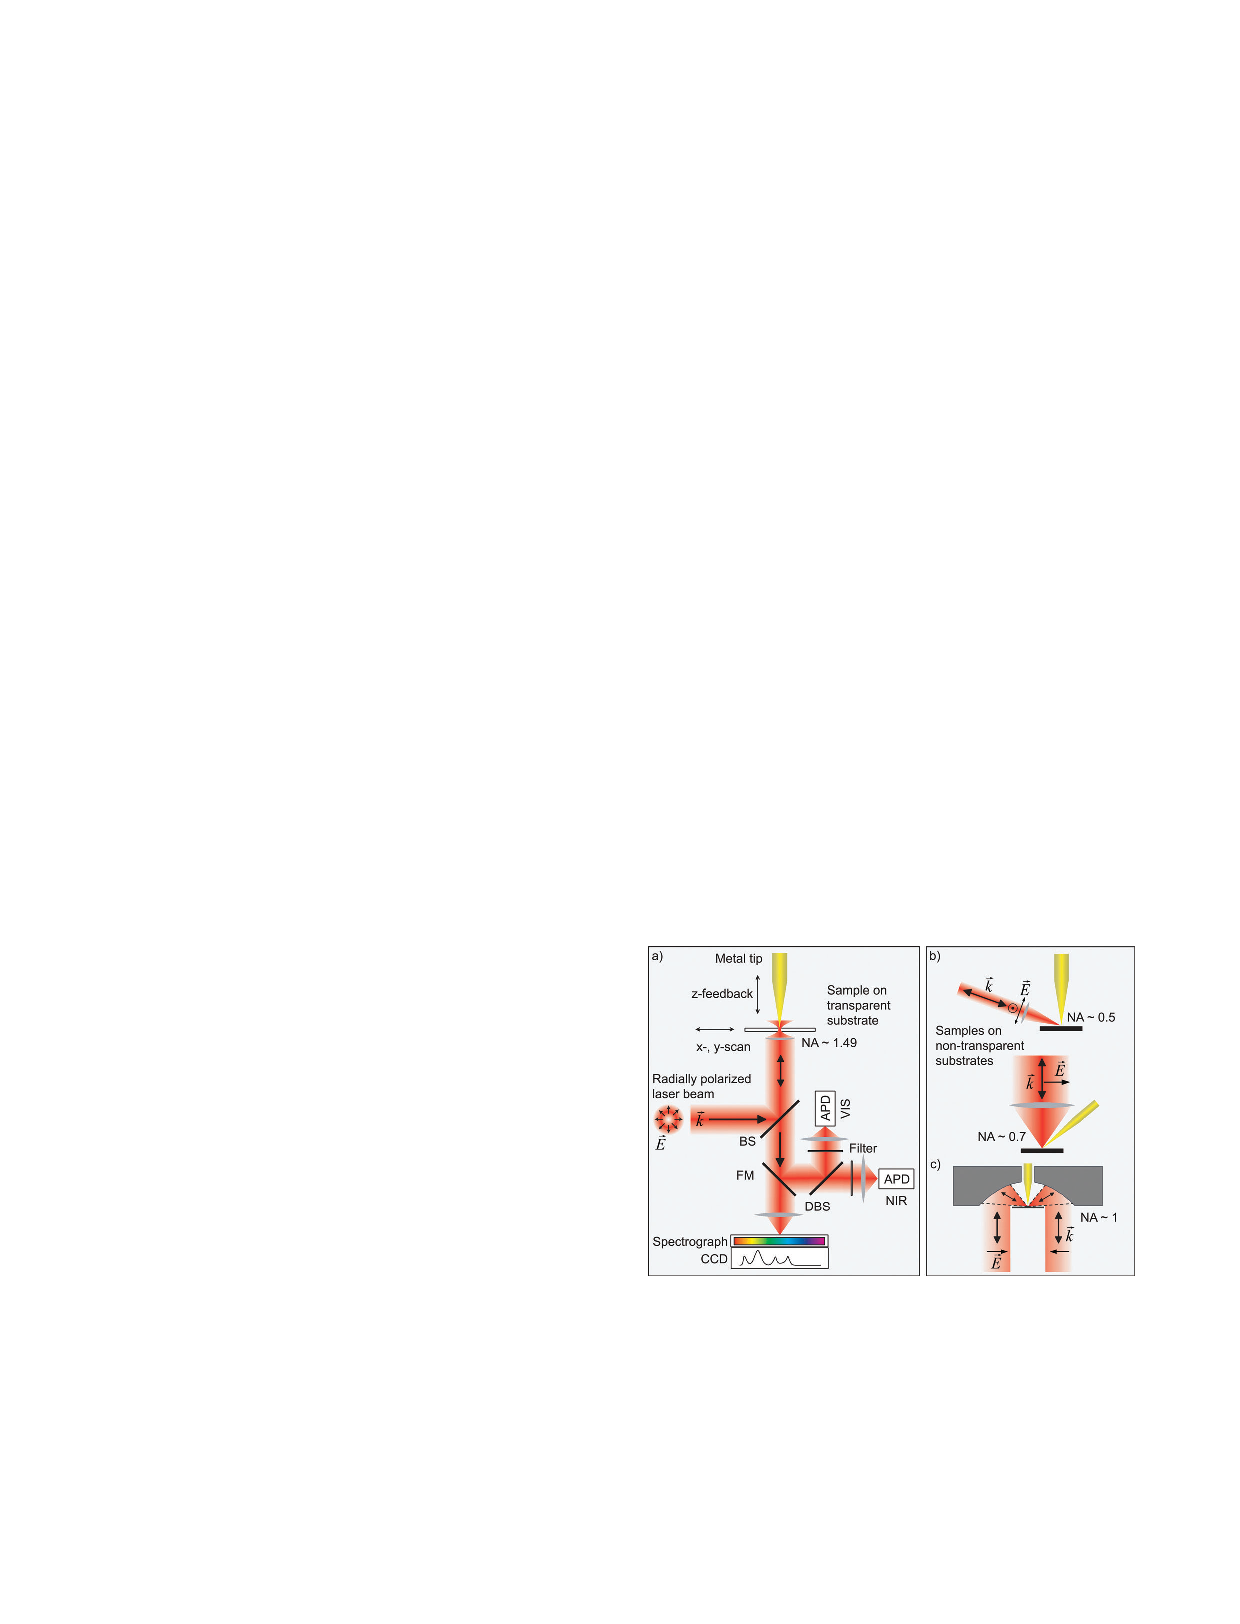
\includegraphics[width=0.6\textwidth]{figures/literature/mauser2014a}
\caption[Typical optical geometries found in TENOM experiments \cite{mauser2014}]{\textbf{Typical optical geometries found in TENOM experiments \cite{mauser2014}.} The most prominent system is the bottom-illumination/back-illumination configuration utilising high-NA objectives. The other main geometry is the side-illumination configuration.}
\label{fig:ters_geometries}
\end{figure}

Since initial investigations, tip-based systems have been designed in two configurations: the side-illumination configuration and the bottom-illumination configuration. Both configurations are shown in \figurename~\ref{fig:ters_geometries}. The specific design of a \gls{tenom} microscope is important as it defines the collection and, more importantly, excitation geometries for the tip.
Side-illumination has been used successfully in a number of cases \cite{mehtani2006, zhang2013, wickramasinghe2014} but suffers generally from far-field scattering overshadowing the near-field scatter. This requires more complex optical geometries to overcome, such as using polarisation-resolved approaches. More recent designs have opted for a top-illumination geometry, in which high \NA\ is achievable by using parabolic reflectors instead of an objective lens \cite{steidtner2007}.
The dominant microscope design is the bottom-illumination configuration using a $\NA>1$ objective to illuminate the tip evanescently whilst masking out the $\NA<1$ illumination in \wvm-space. \gls{tir} of the incident light results in minimal background scatter with only the near-field scattered into a collection aperture. Collection from this geometry can be achieved using either the $\NA<1$ aperture of the high \NA\ objective \cite{hayazawa2001, yeo2006, yeo2007, zhang2013experimental, mino2014, kumar2014} or by using a secondary low \NA\ objective \cite{hayazawa2007, taguchi2009, uetsuki2012}. More importantly, bottom-illumination is advantageous in that it generates evanescent waves capable of coupling to \glspl{spp} in both a metallic substrate and the tip once it is within the near-field. The disadvantage of using bottom-illumination is that it requires semi-transparent samples (enough to transmit and collect sufficient light), which is not always possible.
In general each of these setups is used with a continuous wave laser, although recently ultrafast systems have been employed to extract temporal information from \gls{ters} measurements \cite{klingsporn2013}.

\begin{figure}
\centering
\fcapside[\FBwidth]
{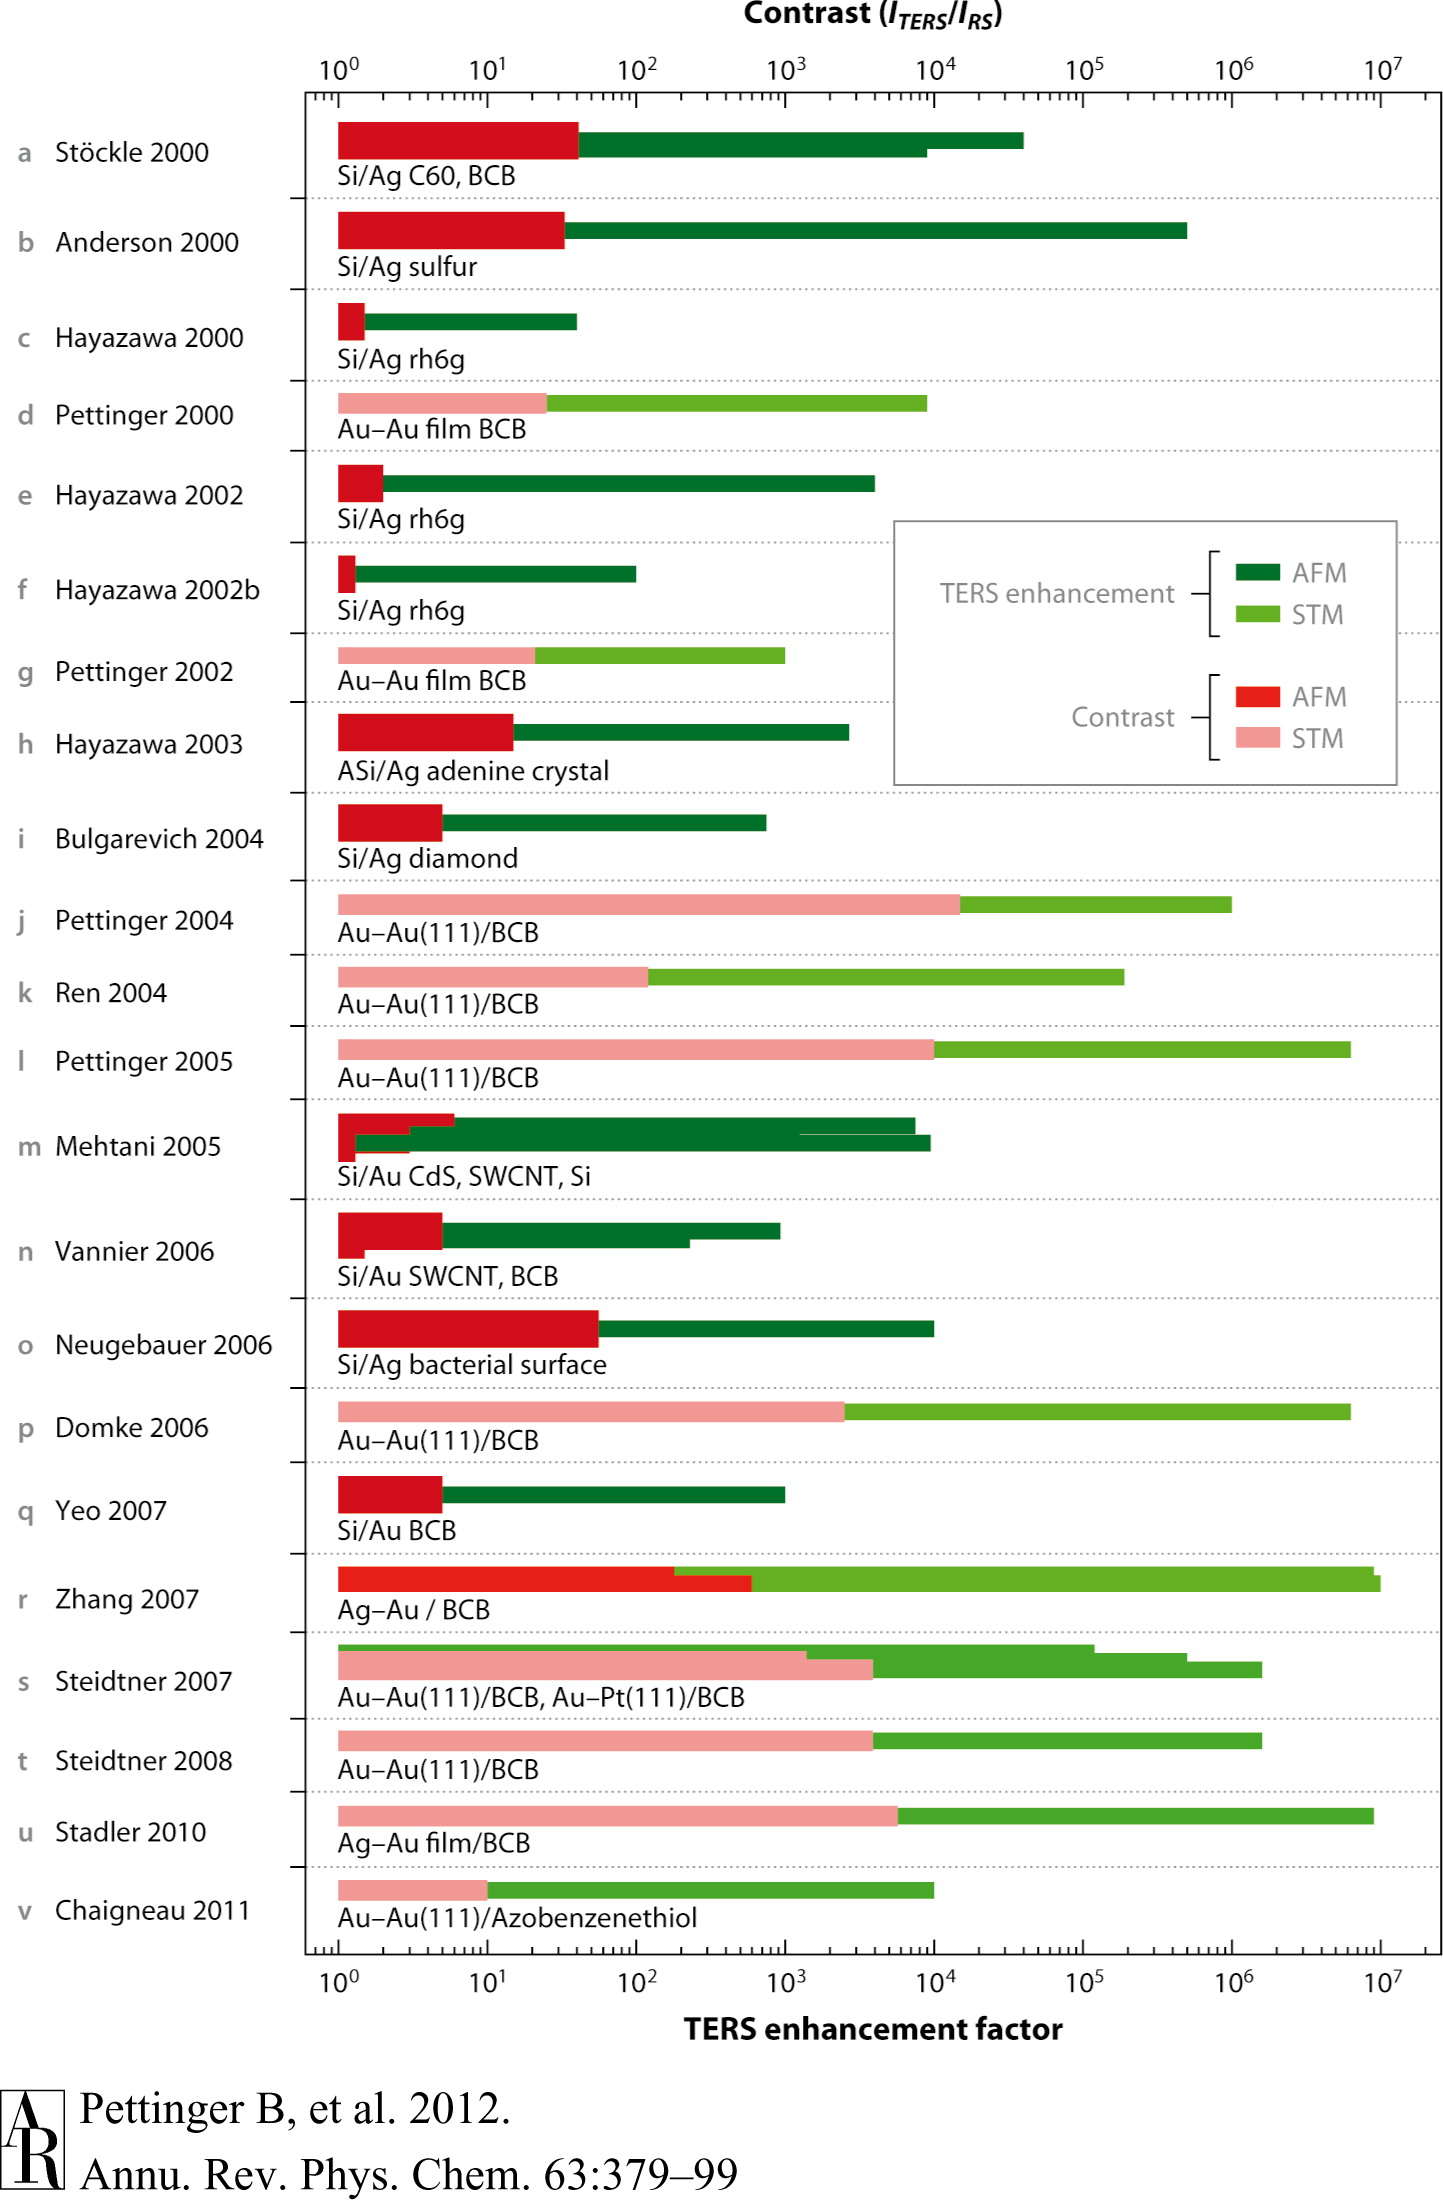
\includegraphics[width=0.7\textwidth, clip=true, trim=0 35 0 0]{figures/literature/pc630379_f8}}
{\caption[Comparison of TERS field enhancements and contrasts reported between 2000 and 2011 \cite{pettinger2012}]{\textbf{Comparison of TERS field enhancements and contrasts reported between 2000 and 2011 \cite{pettinger2012}.} STM tips, likely due to their increased sharpness, outperform AFM tips. Ag tips outperform Au tips. Larger enhancements are observed in systems where there is an underlying thin, noble metallic film. Statistical correlations still remain somewhat weak, showing the current variability in TERS experiments, attributed to irreproducibility of enhancing tips.}
\label{fig:pettinger2012}}
\end{figure}

% Challenges for TERS and comparison between measurements
Since the initial measurements of tip enhancements and plasmons, techniques such as \gls{ters} and \gls{asnom} have become widespread and generally accepted. However, they are currently not reliable enough to be considered as a standard technique. Difficulty controlling the tip near-field is both a result of the irreproducibility of the tip geometry and a lack of understanding of the optical processes governing the enhancement, leading to large variations between reported field enhancements. A selection of TERS field enhancements and contrasts from reports between 2000 and 2011 showing the large variability are shown in \figurename~\ref{fig:pettinger2012}. The current challenges with \gls{tenom} are therefore improving the reproducibility of the near-field enhancement between tips \cite{blum2014, kumar2014, mino2014} and successful electromagnetic modelling and understanding of the tips themselves \cite{}.

% Sharpness and lightning rod effects
From \figurename~\ref{fig:pettinger2012} it is clear that sharper \gls{stm} tips result in larger field enhancements than \gls{afm} tips and comparative studies have shown similar trends \cite{raschke2003, yeo2006, picardi2007}. This is most likely evidence that the lightning rod effect plays a significant role in the near-field enhancement process. Intuition suggests that the sharper profile of solid metallic \gls{stm} tips means a larger lightning rod component compared with metallised \gls{afm} tips, a hypothesis also suggested in recent theory work \cite{zhang2009}. Recent theory suggests that there is a quantum limit in sharpness, set by nonlocal effects, before the field enhancement saturates as structural imperfections become ignored \cite{wiener2012}. Studies have also shown that some large observed enhancement factors can be caused by non-plasmonic artefacts from the tip shaft \cite{ramos2012}. Removal of these artefacts is necessary to recover the actual near-field enhancement \cite{kumar2014}.

% Plasmonic component
\begin{figure}
\centering
\caption[]{\textbf{SEM images of metallised tips showing the granular texture and apex sharpness.} (a)\cite{hayazawa2001, hayazawa2012, mino2014}.}
\label{fig:metallised_tips}
\end{figure}

% Morphology dependence
Variability between similar measurements is not solely due to differences in experimental setup or changes in tip sharpness. A large amount of variability stems from the surface metal morphology. A localised component of the plasmonic tip contribution to the near-field is generally reported to originate from surface roughness that mimics small 10--\SI{50}{nm} \glspl{mnp} \cite{mino2014}. This is similar behaviour to the improvement in \gls{sers} intensity when using a rough metallic film as opposed to a smooth metallic film. Each grain of the coating can act as a point at which photons couple or plasmons radiate, hence a grain located at the apex can plasmonically enhance the near-field. For this reason sharp tips are generally all solid metal or metallised dielectric tips, coated using evaporation (with similar conditions  to metal island deposition) \cite{hayazawa2001, hayazawa2012, mino2014} or chemical reactions \cite{bailo2008}. The disadvantage of this approach to \gls{tenom} is that the randomised tip geometry is not reproducible. Furthermore, granularity is rarely taken into account in theory when trying to explain the mechanisms of \gls{tenom}.

Orientation of the tip with respect to the sample also has been known to influence the near-field enhancement \cite{yeo2006}.

% Material dependence
As with conventional plasmonics, Ag tips generally outperform Au tips under visible light, though these claims strongly depend on the underlying tip material and the morphology of the metallic surface used in the experiment. Plasmon excitation is complicated by the shift induced by refractive index of the underlying tip material in metallised \gls{afm} tips, which can vary drastically between materials such as Si, \ce{SiO2}, and \ce{Si3N4} \cite{picardi2007, taguchi2009}. These high index materials can shift \glspl{spr} into the infrared {\color{red}(\gls{imi} plasmon geometry)} whereas plasmons in bulk metal \gls{stm} tips remain unchanged. Careful consideration must therefore be given when pairing a tip with a laser in order to match the excitation wavelength with the \gls{spr} \cite{yeo2006, yeo2007, cui2007, hayazawa2012}. Numerical simulations further show that resonance positions are highly sensitive to the metallic coating thickness when below the skin depth ($\sim$\SI{40}{nm} for Au), suggesting some experimental variability can originate from inaccuracies in the metallic deposition process \cite{huber2014}. A similar suggestion regarding the optical quality between bulk metal and a metallised dielectric/semiconductor has also been made \cite{picardi2007}.

The majority of previous reports support the hypothesis that tips, in some way, can support both \glspl{spp} and \glspl{lsp}, which contribute to the overall near-field enhancement. However, the dependence on random depositions of rough metal is the main downfall of modern \gls{tenom} and one of the most likely reasons for the lack of reproducibility between measurements. While many recent reports are motivated by the need to improve the reproducibility, typically via tuning the underlying tip dielectric material, very few have achieved this due to a reliance on the grain structure.

Larger enhancements have resulted from coupling with thin metallic substrate films, suggesting the formation of gap plasmons \cite{ren2004, hayazawa2007, yano2007, pettinger2009, uetsuki2012}. Specifically, when a Au tip is paired with a Au substrate the field enhancement is significant increased, moreso than when paired with a Pt surface \cite{ren2004} or a non-metallic surface \cite{} due to better optical polarisability of the substrate. In these cases the Raman enhancement has been shown to rise to $\sim$\num{e7} when illumination is on resonance with the gap mode \cite{uetsuki2012}. % maybe comment more on the mechanism for this excitation as side illumination alone may not be enough i.e. excitation geometry more important than collection.
Theory for the coupling of a Au tip with a Au surface suggests that shifting of a gap resonance should be minimal \cite{downes2006}. Coupling to the localised tip plasmon can be achieved using \gls{spp} excitation on the underlying metallic substrate \cite{hayazawa2007}.

Theory shows increased localisation of the \gls{spp} field even with dielectric substrates \cite{downes2006}.

Finally, variability between similar measurements can stem simply from differences in tip placement, optical setup and the specific illumination/collection geometry or optics used. As tips are rarely characterised there is little traceability between measurements from which to systematically determine the relevant causes for difference.
%However, in this time, further experiments have been carried out to study the plasmonic nature of noble metal tips to understand the near-field around an illuminated tip. Theory has also been developing to complement experiments and successfully model and disentangle the optical response of tip systems.

% Electrical excitation
One final tip-based plasmon excitation mechanism of interest that has been discussed in recent years is electrical excitation. Similar to the use of \gls{eels} in electron microscopy, tunnelling electrons can be used to excite plasmons in an \gls{stm} geometry. Since tips are typically illuminated with a single wavelength of light it becomes difficult to discern plasmonic features hidden in the collected light. Electrical excitation circumvents this limitation as electrons need only to have sufficient energy $eV$ that a portion transferred to the conduction electrons is enough to excite \glspl{sp} with frequencies $h\nu \leq eV$. Electrical excitation also functions to both remove background light contributions to spectra by removing the illumination source.

Using tunnelling current excitation, light has been observed from both the tip-air-metal substrate gap \cite{pettinger2009} and the interface between the metal substrate and its underlying dielectric \cite{wang2011}. Light detected from metal-glass interfaces is leakage radiation from \glspl{spp} on the metal-air interface as the \gls{spp} dispersion crosses the light line ($\wvm_{SPP} = \wvm_{glass} = n\wvm_{air}$, see \figurename~\ref{fig:spp_dispersion}, chapter \ref{ch:theory}). Since light cannot leak from \glspl{spp} at the metal-air interface the detected light must be from gap plasmons between the tip apex and the surface {\color{red}and outcoupling at the curved surface}. It is thought that 95\% of the emission is due to \gls{spp} excitation rather than \gls{lsp} excitation \cite{wang2011}.
% this causes problems with the idea of antenna modes.

Indications of the existence of gap modes between the tip apex and the induced mirror charge distribution in a metallic substrate have been observed in the TERS background of a \gls{stm} tip (side illumination HeNe). Broad background resonances, likely due to electrical excitation of plasmons, redshift as the tip is brought closer to the substrate and follow a dipole-dipole interaction model \cite{pettinger2007, pettinger2009}.

\subsection{Tip Modification, Nanostructuring and Optical Antenna Tips}

% Transitioning the discussion from sharp to nanostructured tips
The mode mismatch caused by the size difference between diffraction-limited light and the nm-scale results in a 3--4 order of magnitude coupling efficiency loss \cite{berweger2010}. As described previously, a \gls{sp} acts as an optical antenna. A good optical antenna has the ability to effectively modify the density of electromagnetic states such that the far-field radiation impedance is efficiently matched with the impedance of a near-field evanescent mode and vice versa \cite{novotny2006, novotny2011}. The antenna opens up scattering pathways between near-field emitters and the far-field by connecting wave states (\wvm-vectors) via new intermediate states (the plasmon). Metallic tips, in their standard form, are not particularly good optical antennae.
{\color{red}The lack of radiative lower order multipolar resonances greatly diminishes the radiative cross section \cite{renger2004}.}
To improve their coupling efficiency, standard sharp tips and their surrounding structures can be modified or nanostructured to introduce such intermediary plasmon states which couple the far-field to the near-field \cite{mauser2014}.

% Grating tips as nanoscale light sources
By patterning a grating onto the side of a conical metallic tip, its apex can be transformed into a nanoscale light source, in which \glspl{spp} excited on the grating propagate to the apex and re-radiate into the near-field \cite{neacsu2010}. Far-field illumination remains spatially separated from the apex suppressing far-field background scatter allowing only scattering of the near-field \glspl{spp} from the apex. The conditions for adiabatic nanofocussing mean that only a single \gls{spp} mode will localise at the apex and radiate. Background-free \gls{ters} signals using the resulting \SI{10}{nm} light source at $\lambda=\SI{800}{nm}$, excited both with continuous wave and ultrafast lasers, have been detected to demonstrate the benefits of using \glspl{spp} to spatially separate the near-field and far-field scatter \cite{berweger2010, berweger2012}.

\begin{figure}[bt]
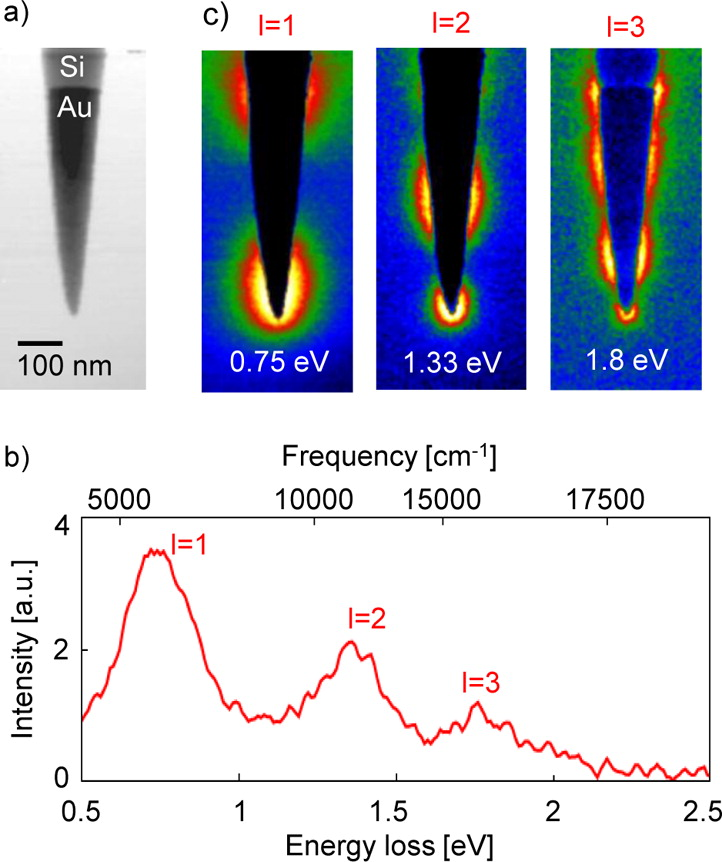
\includegraphics[width=0.45\textwidth]{figures/literature/nl-2012-04289g_0003}
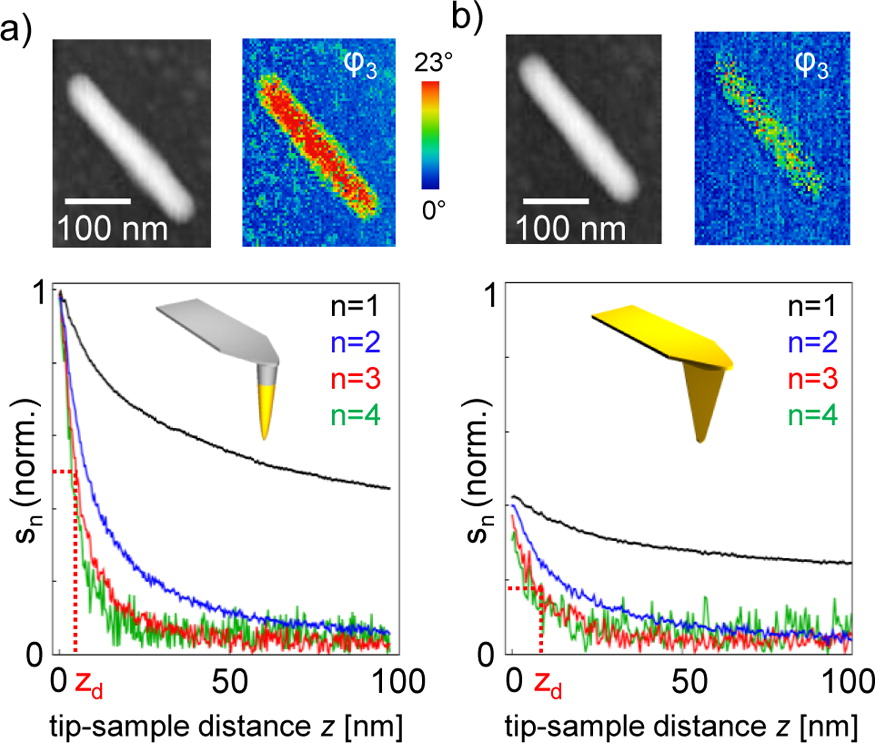
\includegraphics[width=0.45\textwidth]{figures/literature/nl-2012-04289g_0009}
\caption[Comparison between standard Au and nano-antenna AFM tips \cite{huth2013}]{\textbf{Comparison between standard Au and nano-antenna AFM tips \cite{huth2013}.} Nano-antenna tips comprise a Au nanotip on a FIB-cut Si AFM tip. EELS spectra show multipolar rod LSP plasmon modes and scattering measurements demonstrate that nano-antenna tips outperform standard metallised tips.}
\label{fig:huth2013}
\end{figure}

% Nanoantennae tips
To create the necessary \gls{lsp} antenna states for efficient plasmon coupling in the visible spectrum tips must be structured with a distinct, sub-wavelength sized metallic feature. Designs in which the tip is removed and replaced with a planar bow-tie antenna \cite{weber2010} or nano-cone \cite{fleischer2011} have successfully demonstrated improved field enhancement attributed to excitation of a \gls{spr} at the apex. Further evidence for the lack of a plasmonic contribution in sharp metallised tips comes from the comparison between metallised Au tips and Au nanotip probes. A Si tip with the apex replaced by a Au nanotip outperforms a standard Au \gls{afm} tip by 120\% in the side illumination geometry \cite{huth2013}. Similarly cutting the Au coating off past the apex also enables \glspl{lsp} \cite{zou2009}. This level of modification is carried out using FIB machining and is therefore highly controllable, though at the cost of fabrication time and expenses.
Similar structures have been made which also exhibit confined \glspl{spp} \cite{uebel2013}. % check?
To date there are very few reported methods of simply nanostructuring a tip without the need for FIB. A significant amount of time on this project was therefore spent determining a simple approach for chemically producing plasmonic tips.

%\cite{Fleischer2011, Denisyuk2012, Goncharenko2006}

% Introduction to nanostructuring
Recently, nanostructuring of the tip apex has been applied to tune and optimise the optical (plasmonic) properties of nanotips. By reducing the characteristic size of the apex structure, thereby giving it a new, more localised, geometry, light can be more strongly confined in more localised plasmon oscillations, hence the optical antenna properties of a nanotip can be substantially improved. The emergence of new plasmon modes unsupported by regular sharp tips then opens up new mechanisms through which light can be channelled to the nm-scale, such as direct far-field illumination.

\subsubsection{Spherically Nanostructured Tips}

% Spherical nanostructuring
The simplest geometry to impart onto a tip apex is a sub-wavelength metal sphere. By doing so the tip gains \glspl{lsp} similar to those in an isolated spherical \gls{mnp}. The specific \glspl{spr} depend on the sphere attachment method as the base tip structure determines the local dielectric medium adjacent to the \gls{mnp}. Spherical \glspl{mnp} have been successfully nanostructured onto both metallic \cite{savage2012, park2012, kharintsev2013}, semiconductor \cite{umakoshi2012} and insulating \cite{kalkbrenner2004} base substrates, exhibiting clear \glspl{spr} \cite{savage2012}.

\begin{figure}[bt]
\centering
\begin{subfigure}[t]{0.35\textwidth}
	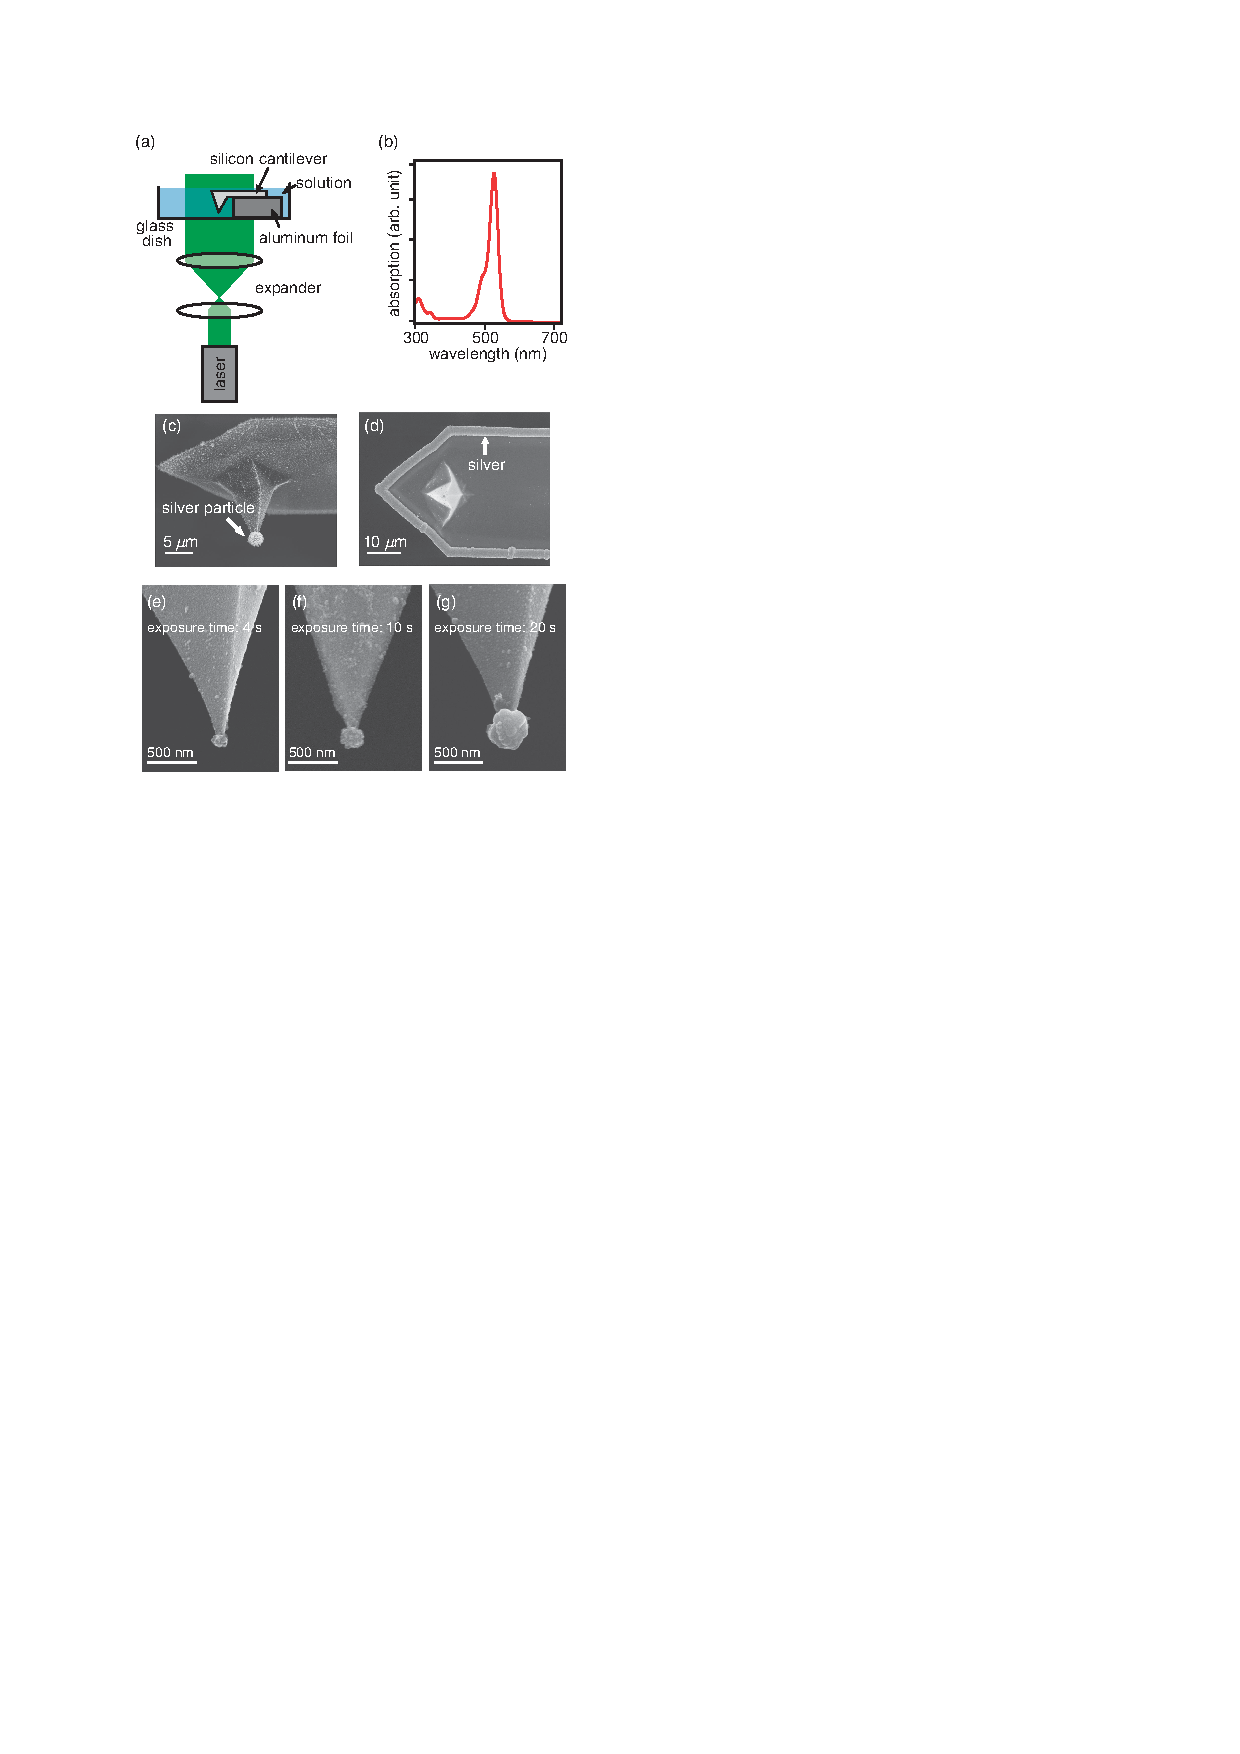
\includegraphics[width=\textwidth, clip=true, trim=0 0 0 130]{figures/literature/umakoshi2012a}
	\caption{Photochemical fabrication of AgNP-tipped AFM probes}
\end{subfigure}
%\begin{subfigure}[t]{0.4\textwidth}
%	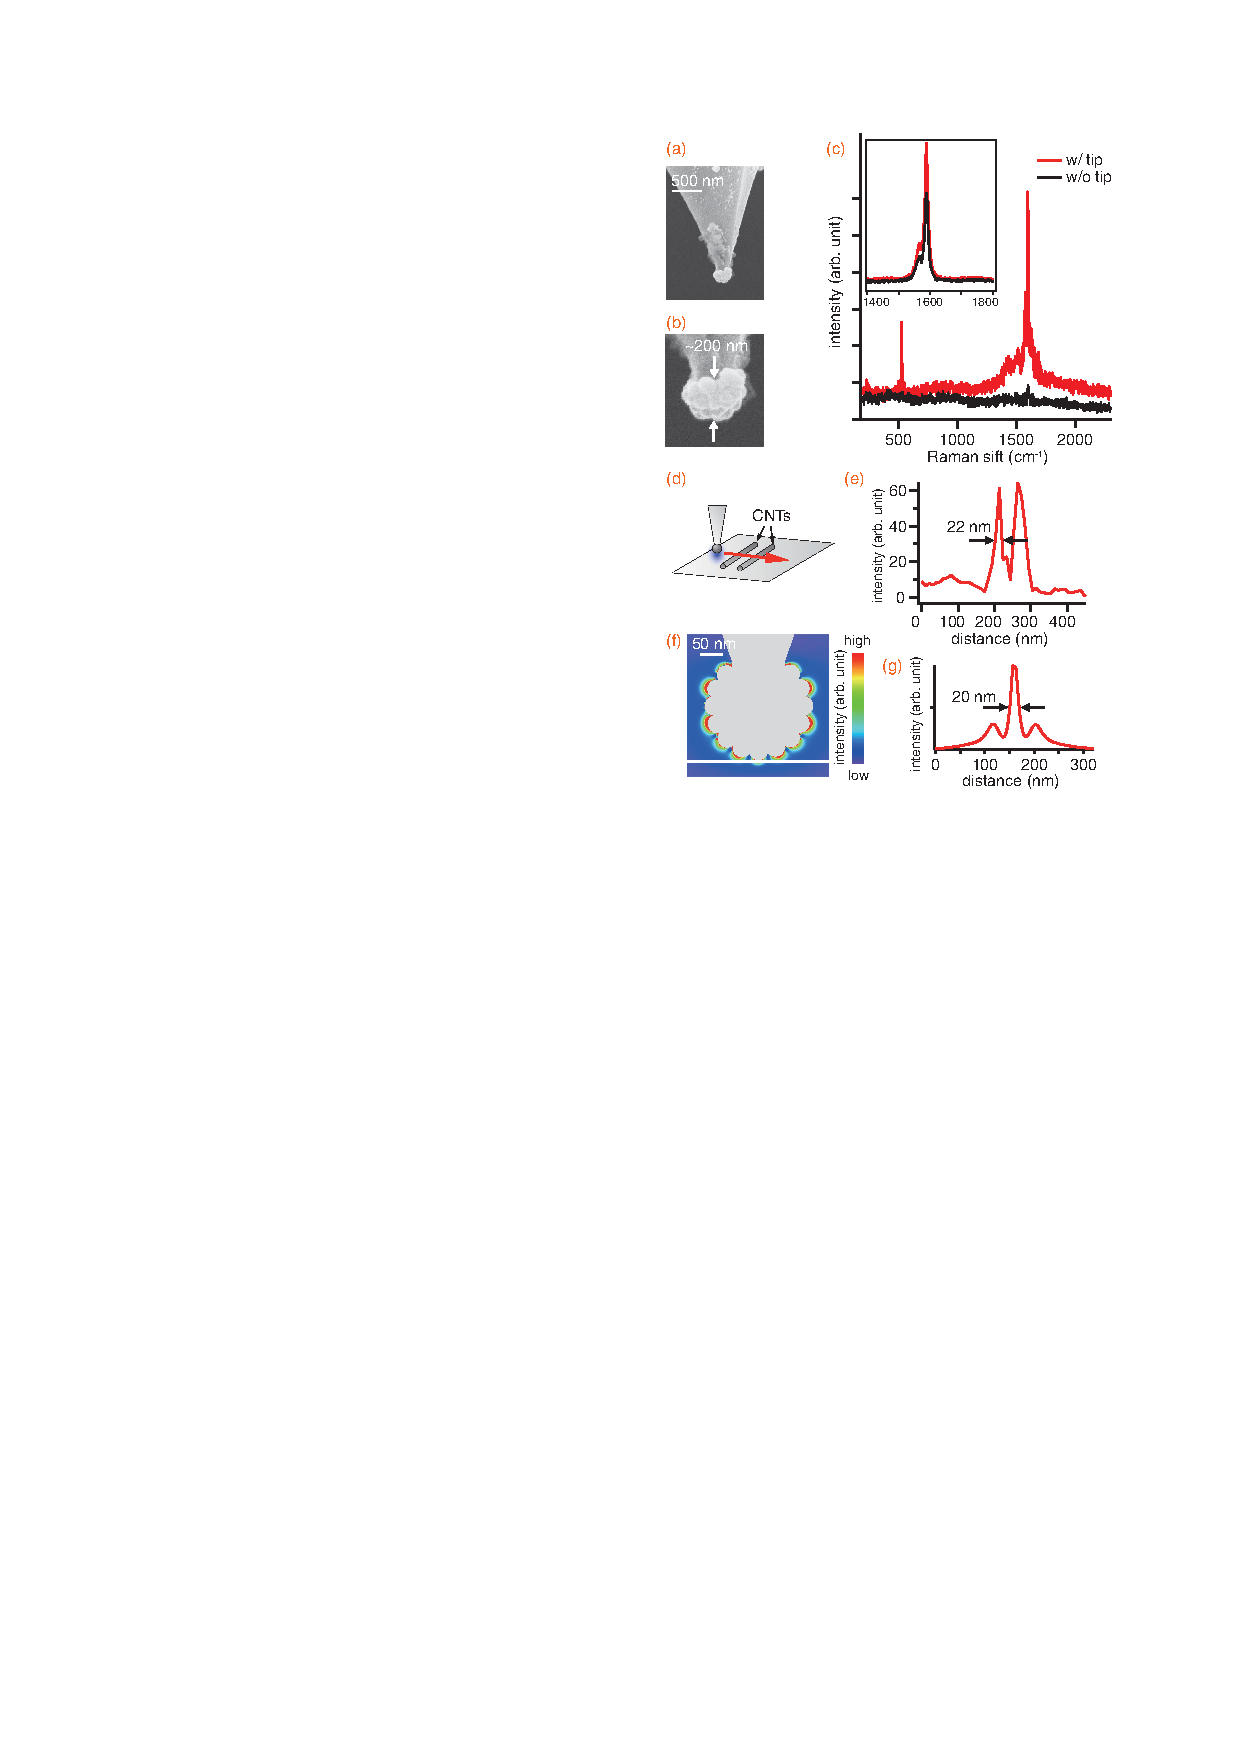
\includegraphics[width=\textwidth, clip=true, trim=0 155 0 0]{figures/literature/umakoshi2012b}
%	\caption{TERS measurements and numerical simulations of AgNP-on-Si tips.}
%\end{subfigure}
\caption[Photochemically fabricated AgNP-on-Si tips for TERS \cite{umakoshi2012}]{\textbf{Photochemically fabricated AgNP-on-Si tips for TERS \cite{umakoshi2012}.} Field enhancement is increased $\sim 20 \times$ compared with sharp Ag tips when using \SI{488}{nm} illumination with a 1.4\,NA objective in an inverted microscope.}
\label{fig:umakoshi2012}
\end{figure}

% Non-metallic attachment
Non-metallic spherical tips on AFM probes have been created using methods such as vacuum-processing diamond-like carbon growth (NanoTools B-series) and AFM droplet pick-up \cite{}. These nanotips can then be made plasmonic through evaporation of a metallic coating.
% Metallic attachment
Other methods directly focus on structuring the apex with a solid metallic structure rather than using a post-fabrication coating.
% Concept and methods of attachment
The concept of metallic spherical nanoparticle attachment has been reported numerous times over the last decade \cite{gan2007}, beginning with the use of fibres as mounting structures \cite{kalkbrenner2001, barsegova2002, sqalli2002, kawata2003} and progressing onto the use of SPM tips \cite{umakoshi2012, hayazawa2012, park2012, okamoto2001, vakarelski2006, cheng2013}.
% Example figures
Examples of nanotips modified with metallic spherical nanostructures are shown in \figurename~\ref{fig:umakoshi2012}.

\begin{figure}[bt]
\centering
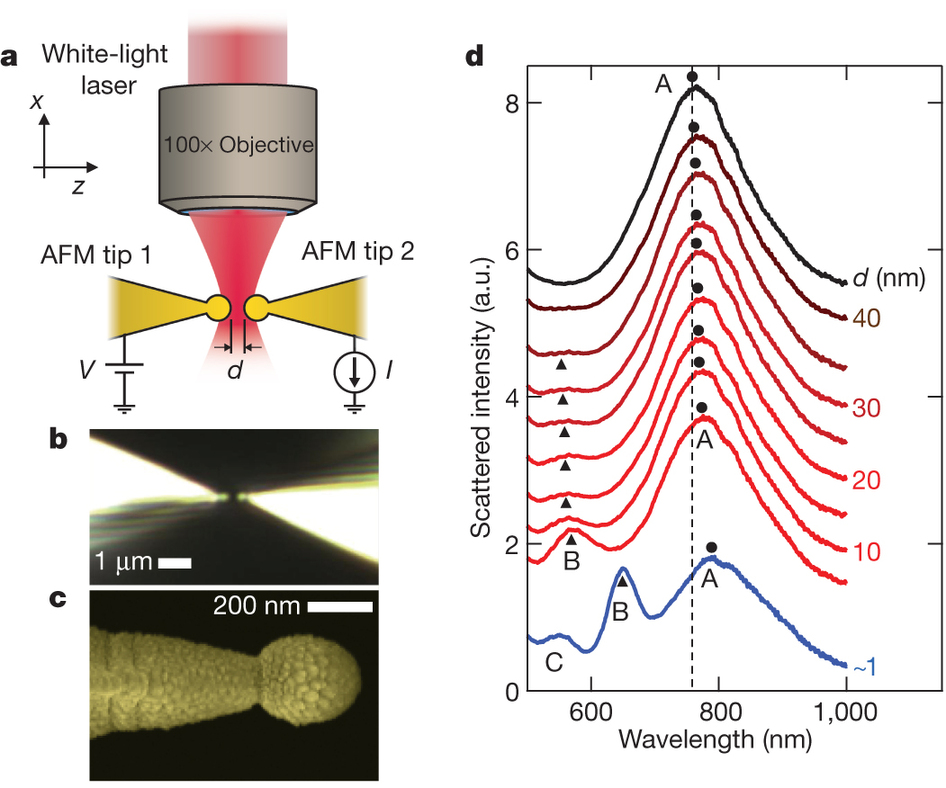
\includegraphics[width=0.65\textwidth, clip=true, trim=0 0 0 40]{figures/literature/nature11653-f1-2}
\caption[Experimental evidence of spherical tip plasmons and their dynamic coupling into the quantum regime of plasmonics \cite{savage2012}]{\textbf{Experimental evidence of spherical tip plasmons and their dynamic coupling into the quantum regime of plasmonics \cite{savage2012}.} Spherical tips are Au-coated NanoTools B150 AFM probes (\SI{150}{nm} radius of curvature), selected to minimise sensitivity to axial tip-tip alignment, to increase the scattered signal levels, and support higher-order plasmonic cavity modes in the visible spectrum. Resonances are far-field excited using a supercontinuum laser source in a side-illumination configuration. Separation-dependent coupling between two spherical tips confirms plasmonic behaviour.}
\label{fig:savage2012a}
\end{figure}

% Direct measurement
Plasmon resonances in spherical tips have been observed in the far-field \cite{savage2012}, with coupling between plasmons used to confirm plasmonic behaviour.
% TERS
Furthermore a $20\times$ increase in field enhancement has been measured when using a photochemically-fabricated spherical AgNP-on-Pt tip compared with a sharp Ag tip \cite{umakoshi2012}. The increase in field enhancement also comes with an increase in {\color{red}resolution/spatial localisation}.

% Other geometries
Nanostructuring tips with other geometries has also led to an order of magnitude increase in field enhancement, attributed to LSP excitation. Electrochemical etching \cite{kharintsev2013}, FIB machining \cite{maouli2015}, selective deposition \cite{zou2009} and grafting \cite{huth2013} have successfully been used to create nanotips which are good optical antennae, especially when illuminated on resonance. Scattering resonances have been directly measured on a subset of these tips \cite{zou2009, maouli2015} while others use the field enhancement at common laser wavelengths as a measurement of antenna quality \cite{kharintsev2013}.

\cite{ichimura2009, taguchi2009, vanschrojensteinlantman2012, angulo2011, sonntag2014}
% Techniques to improve TERS such as stimulated vs. spontaneous Raman \cite{wickramasinghe2014}. Picosecond pulses \cite{klingsporn2014}
% Still to read Ichimura2009, Sch�fer2013, Pettinger2009, Cherukulappurath2013, ?Zhang2013?, Taguchi2009, Yang2014, Steidtner2007, Schrojenstein2012, ?Zhang2014?, Angulo2011, Picardi2007, Uebel2013, ?Meng?, Sonntag2014, Lindquist2013, Mino2014, Pettinger2007, Ren2004, Hayazawa2007, Park2012, Downes2006, Yano2007, El-Khoury2014, Pettinger2009, Cajko2006
% Also note that thicknesses below skin depth on tips could in theory create a resonant structure since there is a dielectric on both sides.

To date there has been very little work done to reliably produce and characterise the optics of spherically nanostructured tips. Furthermore, there is still work needed to similarly measure the optical response of sharp tips, comparing them directly and quantitatively with nanostructured tips. This project focusses on developing a simple method for producing plasmonic tips with understood far-field optical responses. The comparison with sharp metallic tips can then be made and plasmonic tips applied in both fundamental studies and near-field enhancement.

\end{document}